\section{Architektur}\label{sec:architecture}

fulib.org verwendet eine einfache Architektur bestehend aus Frontend, Backend und Datenbank.
Da es sich um eine Webanwendung handelt, wird das Frontend im Browser ausgeführt.
Öffnet man die Seite, werden die benötigten HTML-, JavaScript- und CSS-Dateien vom Backend heruntergeladen und im Browser angezeigt.
Aus Sicht des Backends sind dies statische Ressourcen.
Sämtlicher Datenaustausch in der Webanwendung geschieht dann über REST/HTTP-Anfragen an das Backend.
Dabei wird JSON als Datenformat verwendet.
Für die persistente Datenspeicherung von Anfragelogs, Aufgabenblättern, Lösungen, Kursen und Kommentaren kommt eine Mongo\cite{mongodb}-Datenbank zum Einsatz.
Die Kompilierung und Ausführung von Scenarios wird durch Anbinden des Scenario- und Java-Compilers sowie eines JUnit Runners bewerkstelligt.
Abbildung~\ref{fig:website-architecture} gibt einen Überblick über die verschiedenen Komponenten,
die es der Webseite ermöglichen, ihre Funktionalität bereitzustellen.
Im folgenden Abschnitt wird näher erläutert, wie diese zusammenwirken.

\begin{figure}
    \centering
    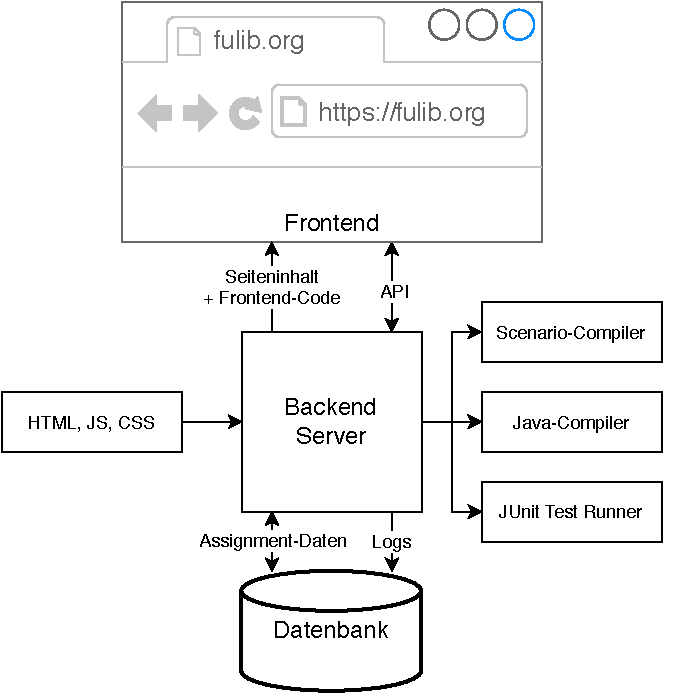
\includegraphics[width=0.5\textwidth]{chapter/fulib.org/img/architecture.pdf}
    \caption{Architektur von fulib.org}
    \label{fig:website-architecture}
\end{figure}

\subsection{Frontend}\label{subsec:frontend}

Das Frontend von fulib.org ist mit dem Angular~\cite{angular}-Framework implementiert.
Dieses gibt insbesondere eine Architektur vor, die Business Logic (Services) von UI-Logik (Components) trennt.
Services sind beispielsweise dafür zuständig, mit dem Backend Daten auszutauschen,
während Komponenten sich mit deren Darstellung befassen.
Letztere haben weiterhin als wiederverwendbare Elemente Bedeutung.
Sie ermöglichen es, gemeinsame Funktionalität zu verkapseln und an mehreren Orten zu verwenden.
Im Kontext der Assignments ist beispielsweise die Task-Liste eine Komponente, die auf mehreren Seiten zum Einsatz kommt.
Da Komponenten nur einmal implementiert und beliebig wiederverwendet werden können,
kann die Oberfläche konsistent und fehlerfrei gehalten werden.

Das Aussehen der Oberfläche von fulib.org basiert auf Bootstrap~4~\cite{bootstrap}.
Das CSS-Framework gibt vielen HTML-Elementen wie Buttons oder Eingabefeldern ein modernes Aussehen.
Weiterhin gibt ermöglicht es die einfache Anordnung von Elementen, die sich an verschiedene Bildschirmgrößen anpassen kann.
So ist fulib.org ohne großen Entwicklungsaufwand auch auf Smartphones o.ä.\ übersichtlich.
Bei dem im Footer einstellbaren Nachtmodus (Darkmode) handelt es sich um die Bootstrap-Darkmode~\cite{bootstrap-darkmode}.
Diese Eigenentwicklung passt die Farbgebung von Bootstrap so an, dass alle normalerweise weißen oder hellen Elemente in schwarz- bzw.\ grautönen erscheinen.
Dies schont bei dunkleren Lichtbedingung wie etwa abends das Auge.

Die Editorfenster für Scenarios und Java-Code sind mit der CodeMirror~\cite{codemirror}-Bibliothek implementiert.
Diese bietet einen Editor, der Syntaxhighlighting für viele Programmiersprachen unterstützt.
Mit Themes kann die Farbgebung angepasst werden, was auf fulib.org beim Wechsel in den Nachtmodus zu beobachten ist.
Zudem unterstützt der Editor eine Reihe von Addons, die zusätzliche Funktionalität einbringen können.
Beispielsweise können mit dem Lint-Addon Fehlermeldungen im Editor hervorgehoben werden.
Es ist geplant, dies im Scenario-Editor einzusetzen.

\subsection{Backend}\label{subsec:backend}

Bei dem Backend von fulib.org handelt es sich um einen einfachen HTTP-Server.
Dieser ist zustandslos, arbeitet also nach dem REST-Prinzip.
Dabei sind die Hauptaufgaben die Auslieferung des Frontends,
die Ausführung von Scenarios,
sowie die Kommunikation mit der Datenbank im Kontext von Assignments.

Das Ergebnis des Buildprozesses des Frontends sind statische HTML-, JavaScript- und CSS-Dateien.
Diese werden vom Backend auf Anfrage eines Browsers unverändert an diesen übermittelt.
Anders als bei dynamisch bzw.\ serverseitig generierten Webseiten hat dies den Vorteil,
dass der Ressourcenaufwand des Servers sehr gering ist.
Auch lassen sich die statischen Ressourcen sehr gut cachen,
beispielsweise in einem zwischenstehenden Cache oder im Browser.
Dies kann mit Ausnahme vom ersten Besuch der Seite die Ladezeiten erheblich verkürzen.
Jedoch steigt der Aufwand auf Client- bzw.\ Browserseite,
der nach Herunterladen der statischen Dateien das JavaScript ausführen muss, um den Webseiteninhalt aufzubauen.
Dies kann bei weniger leistungsfähigen Geräten wie älteren Smartphones für längere Verzögerungen sorgen.

Die Ausführung der Scenarios delegiert an die drei zuständigen Tools,
den Scenario- und Java-Compiler und JUnit.
Der Server schreibt zunächst den über die API empfangenen Text in eine Datei in einem temporären Ordner.
Daraufhin wird der Scenario-Compiler in diesem Ordner ausgeführt,
der die Java-Dateien sowie das Klassendiagramm generiert.
Mit dem Java Compiler wird der Java-Code dann kompiliert und die entstehenden Klassen dynamisch geladen.
Das JUnit-Framework bietet eine Schnittstelle zum Ausführen der Test-Klassen,
wodurch das Testergebnis sowie die Objektdiagramme entstehen.
Die Ausgaben der drei Tools werden dabei protokolliert, um einen Teil der Antwort zu bilden.
Der temporäre Ordner wird daraufhin nach Diagramm- und Java-Dateien durchsucht.
Erstere werden unter Anwendung einer geeigneten Kodierung in die API-Antwort übernommen.
Aus letzteren werden relevante Methodenrümpfe durch einen einfachen Parser extrahiert.

Die Kommunikation mit der Datenbank ist besonders bei Assignments und verwandter Funktionalität relevant.
Alle dafür zuständigen Endpunkte lesen entweder Daten aus der Datenbank oder erzeugen neue Datensätze in dieser.
Beim Anlegen ist das Anfrageformat stets JSON;
der Server konvertiert dies zunächst in sein eigenes Datenmodell.
Dieses wird beim Speichern in der Datenbank in deren natives Format konvertiert.
Umgekehrt ist es bei Leseanfragen, bei denen der Server Anfragen an die Datenbank stellt,
deren Ergebnis in sein Datenmodell konvertiert und dies als JSON in der Antwort zurückgibt.
Das Backend ist bei sämtlichen Anfragen für die Prüfung von Tokens zur Autorisierung zuständig,
wobei sichergestellt wird, dass keine Daten bei nicht befugten Anfragen preisgegeben werden.
Insbesondere wird diese Prüfung nicht im Frontend durchgeführt,
da sonst ein Angreifer manuell die Server-API ansprechen und ausnutzen könnte.
